% !TeX root = 控制工程基础笔记.tex
\chapter{控制系统的频率特性}
\label{sec:控制系统的频率特性}

时域分析直观，但要得到高阶系统的时间响应必须解高阶微分方程，计算繁琐；而系统对正弦输入的稳态响应却具有一个非常规整的性质——输出仍是同频率的正弦信号，只是幅值和相位随频率而变。这一性质使我们可以用\textbf{频率特性}描述系统，并借助曲线和作图方法分析稳定性与性能。本章先建立频率特性的概念，后续将用它研究系统的稳定性（奈氏判据）与校正。

\section{频率响应与频率特性}
\label{sec:频率响应与频率特性}

\begin{definition}[频率响应与频率特性]
线性定常系统对正弦输入的稳态响应，称为\textbf{频率响应}；稳态输出与输入的幅值之比、相位之差随频率 $\omega$ 变化的规律，称为系统的\textbf{频率特性}。对传递函数为 $G(s)$ 的稳定线性定常系统，频率特性记作 $G(\mathrm{j}\omega)$，即
\begin{equation}
G(\mathrm{j}\omega)=G(s)\big|_{s=\mathrm{j}\omega}
=\left|G(\mathrm{j}\omega)\right|\mathrm{e}^{\mathrm{j}\varphi(\omega)},
\label{eq:频率特性}
\end{equation}
其中 $\left|G(\mathrm{j}\omega)\right|$ 称为\textbf{幅频特性}，$\varphi(\omega)=\angle G(\mathrm{j}\omega)$ 称为\textbf{相频特性}。
\end{definition}

\subsection{频率不变性}
\label{sec:频率不变性}

频率特性的物理本质是\textbf{放大与移相}。设系统稳定、传递函数为 $G(s)$，输入正弦信号
\[
x_{\mathrm{i}}(t)=A\sin\omega t,
\]
其象函数为 $X_{\mathrm{i}}(s)=\dfrac{A\omega}{s^{2}+\omega^{2}}$。输出象函数为
\begin{equation}
X_{\mathrm{o}}(s)=G(s)\cdot\frac{A\omega}{s^{2}+\omega^{2}}.
\label{eq:正弦输出象函数}
\end{equation}
设 $G(s)$ 的极点为 $s_{j}$（均位于左半平面），$G(\mathrm{j}\omega)$ 存在，则对式~\eqref{eq:正弦输出象函数} 作部分分式展开并求反变换，输出可写成
\begin{equation}
x_{\mathrm{o}}(t)=\underbrace{\sum_{j}c_{j}\mathrm{e}^{s_{j}t}}_{\text{瞬态分量（}t\to\infty\text{ 时衰减为零）}}
+\underbrace{\left|G(\mathrm{j}\omega)\right|A\sin\left(\omega t+\varphi(\omega)\right)}_{\text{稳态分量}},
\label{eq:正弦全响应}
\end{equation}
其中 $\varphi(\omega)=\angle G(\mathrm{j}\omega)$。当 $t\to\infty$ 时瞬态分量衰减为零，只剩稳态分量
\begin{equation}
x_{\mathrm{os}}(t)=\left|G(\mathrm{j}\omega)\right|A\sin\left(\omega t+\varphi(\omega)\right).
\label{eq:正弦稳态响应}
\end{equation}

\begin{property}[频率不变性]
线性定常系统在正弦输入下，其稳态输出是\textbf{与输入同频率}的正弦信号，只是振幅变为输入的 $\left|G(\mathrm{j}\omega)\right|$ 倍，相位比输入滞后（或超前）$\varphi(\omega)$。频率保持不变，故称\textbf{频率不变性}（也叫保频性）。
\end{property}

\begin{remark}
稳态输出中已经含有 $\omega$，说明只有改变频率才能看到不同的放大和移相效果。把幅值比和相位差分别看成频率的函数，就得到了幅频特性和相频特性；两者一起构成了系统在频域的「指纹」。频率特性与传递函数本质上是同一个东西：传递函数是 $s$ 域的描述，频率特性是它在虚轴 $s=\mathrm{j}\omega$ 上的取值。
\end{remark}

\begin{definition}[广义开环系统]
在对系统作频域分析时，常把前向通道 $G(s)$ 与反馈通道 $H(s)$ 的乘积称为\textbf{广义开环传递函数}（简称开环传递函数），记作
\begin{equation}
G_{k}(s)=G(s)H(s).
\label{eq:广义开环传递函数}
\end{equation}
相应地，闭环系统为反馈连接，其闭环传递函数为 $\Phi(s)=\dfrac{G(s)}{1+G(s)H(s)}$（见式~\eqref{eq:闭环传递函数}）。开环频率特性 $G_{k}(\mathrm{j}\omega)=G(\mathrm{j}\omega)H(\mathrm{j}\omega)$ 是后续奈氏判据、伯德图分析与系统校正的主要研究对象。
\end{definition}

\subsection{频率特性的图示方法}
\label{sec:频率特性的图示方法}

频率特性 $G(\mathrm{j}\omega)$ 是频率 $\omega$ 的复变函数，为便于工程使用，通常用图形表示，常用的有三种：

\begin{itemize}
\item \textbf{幅相频率特性曲线（Nyquist 图）}：当 $\omega$ 从 $0$ 变化到 $+\infty$ 时，$G(\mathrm{j}\omega)$ 在复平面上描出的轨迹。曲线上每一点都对应一个频率，同时给出该频率下的幅值和相位。
\item \textbf{对数频率特性曲线（Bode 图）}：由对数幅频特性和对数相频特性两条曲线组成，横轴为 $\lg\omega$；纵轴分别为 $20\lg\left|G(\mathrm{j}\omega)\right|$（单位 dB）和 $\varphi(\omega)$（单位度）。对数作图能把串联环节的乘除化为加减，是工程上最常用的形式。
\item \textbf{对数幅相频率特性曲线（Nichols 图）}：以 $\varphi(\omega)$ 为横轴、$20\lg\left|G(\mathrm{j}\omega)\right|$ 为纵轴的曲线，多用于校正设计。
\end{itemize}

\begin{figure}[H]
\centering
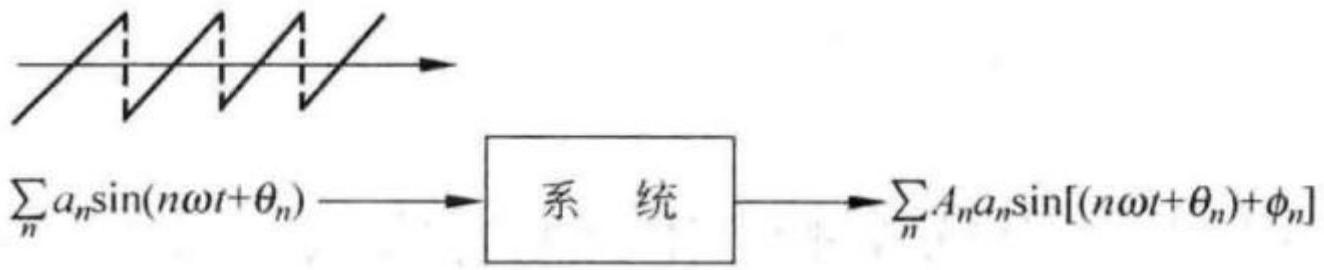
\includegraphics[width=0.85\textwidth]{figures/频率特性示意图.jpg}
\caption{线性系统对正弦输入的稳态响应（频率不变性）}
\label{fig:频率特性示意图}
\end{figure}

\begin{tipbox}[下一节做什么]
本章建立了「正弦输入 $\to$ 同频正弦稳态输出」这一基本事实，并给出了频率特性的定义与三种图示方法。下一节将具体讨论\textbf{奈氏判据}：把开环频率特性 $G_{k}(\mathrm{j}\omega)$ 画在复平面上，依据它包围临界点 $(-1,\mathrm{j}0)$ 的情况来判断闭环系统的稳定性，从而把稳定性问题转化为一次几何计数。
\end{tipbox}
